%-----------------------------------------------------------------------------%
\chapter{\babDua}
%-----------------------------------------------------------------------------%
Bab ini akan menjelaskan sekilas tentang \textit{computational drug discovery}, apa itu \textit{cloud computing} , dan Docker sebagai platform virtualisasi komputer. 
%-----------------------------------------------------------------------------%
\section{\textit{Drug dicovery}}
%-----------------------------------------------------------------------------%
\hspace{0.5cm}\textit{Drug discovery} adalah suatu proses menemukan kandidat obat yang berpotensial. Aktivitas tersebut merupakan misi utama yang diemban oleh perusahaan farmasi bidang obat - obatan untuk mengerti cara kerja penyakit sehingga dapat ditemukan obat / penyembuh yang aman untuk dikonsumsi oleh pasien. Para peneliti berusaha memahami cara kerja penyakit pada level gen dan protein. Dalam hal ini, terdapat istilah "target", dimana calon potensial obat dapat bereaksi. Berikut merupakan tahapan - tahapan yang dilewati dalam \textit{Drug discovery} \cite{Drugdiscovery} :
\begin{itemize}
	\item Validasi target
	\item Menemukan molekul yang dapat berinteraksi dengan target
	\item Melakukan uji coba terhadap senyawa hasil interaksi tersebut untuk memastikan keamanan dan keberhasilan dari senyawa tersebut
	\item Mendapatkan izin untuk membuat dan mendistribusikan obat tersebut 
\end{itemize}
Estimasi waktu yang diperlukan dalam proses ini adalah 10 - 14 tahun \cite{Drugdiscovery2}. Secara lebih jelas tahapan yang dilakukan dalam \textit{drug discovery} :

\begin{itemize} 
\item{\textbf{\textit{Pre-discovery}}}
%-----------------------------------------------------------------------------%
\\Pada tahapan ini peneliti bekerja untuk memahami penyakit. Dimulai dari bagaimana gen berubah sehingga mempengaruhi protein yang di\textit{encode}, bagaimana protein tersebut berinteraksi dengan sel - sel hidup sekitar, bagaimana lapisan sel - sel hidup yang terpengaruh berubah dan bagaiamana penyakit tersebut mempengaruhi pasien secara keseluruhan. Hasil yang didapat dalam tahapan ini merupakan kunci utama dalam menyelesaikan permasalahan (penyakit).


\item{\textbf{\textit{Target Identification}}}
%-----------------------------------------------------------------------------%
\\Setelah peneliti memahami penyakit dan elemen yang mempengaruhi penyakit tersebut, peneliti akan menentukan "target" untuk calon obat baru. Target merupakan \textit{single} molekul, seperti gen atau protein yang terkait dengan penyakit tersebut. Target tersebut harus dipastikan bersifat \textit{drugable}, dimana dapat berinteraksi dengan dan dipengaruhi oleh molekul obat. 

\item{\textbf{\textit{Target Validation}}}
%-----------------------------------------------------------------------------%
\\Setelah target tersebut diidentifikasi, peneliti perlu memastikan apakah target tersebut benar - benar terlibat dalam penyakit dan bersifat \textit{drugable}. Peneliti mengujicobakan target tersebut ke dalam sel hidup dan hewan uji coba lab.

\item{\textbf{\textit{Drug Discovery}}}
%-----------------------------------------------------------------------------%
\\Dengan berbekal pengetahuan yang didapat pada tahap sebelumnya, para peneliti akan mencari molekul yang akan bereaksi dengan target yang telah ditemukan sebelumnya dan mengembalikan efek yang disebabkan oleh target tersebut. Tahapan ini memakan separuh hingga sebagian besar waktu dari \textit{drug discovery} tersebut. Molekul yang ditemukan dalam tahapan ini bisa menjadi suatu obat baru. Beberapa cara untuk mendapatkan molekul tersebut :
\begin{itemize}
	\item \textbf{\textit{nature}}, dengan memanfaatkan alam dan ikatan yang terkandung didalamnya. Sebagai contoh pemanfaatan bakteri dalam pengobatan.
	\item \textbf{\textit{De Novo}}, dengan ilmu kimia dan pemanfaatan teknologi komputer, pembentukan molekul dari awal dengan memanfaatkan komputer untuk memodelkan molekul tersebut dan memprediksi sifat dari molekul tersebut.
	\item \textbf{\textit{High-throughput Screening}}, dengan memanfaatkan tenaga komputasi komputer, memungkinkan untuk membandingkan ratusan ikatan molekul dengan target. Ikatan yang diperoleh dari perbandingan tersebut akan dipelajari kembali dikemudian hari untuk dipastikan kebenarannya.
	\item \textbf{\textit{Biotechnology}}, dengan teknologi ini para peneliti dapat membuat mensimulasikan suatu organisasi kehidupan untuk menghasilkan molekul yang dapat melawan target.
\end{itemize}
\end{itemize}

\section{\textit{Computational Drug discovery}}
%-----------------------------------------------------------------------------%
\hspace{0.5cm}Waktu yang dibutuhkan dalam proses \textit{drug discovery} cukup lama. Tidak hanya itu, proses ini juga sangat beresiko dan membutuhkan dana yang besar \cite{Drugdiscovery2}. Walaupun demikian, investasi dana dalam \textit{drug discovery} juga berkembang pesat. Namun, investasi tersebut tidak diiringi dengan hasil yang proporsional dengan investasi tersebut. Hal ini disebabkan oleh rendahnya efektivitas dan tingginya kemungkinan kegagalan dalam \textit{drug discovery}. Beberapa pendekatan telah dilakukan dalam meningkatkan efektivitas, salah satu cara tersebut adalah CADD (\textit{Computer Aided Drug Design}). Dengan begitu, penekanan biaya dan siklus waktu penemuan obat juga semakin cepat. Dalam CADD, komputer digunakan sebagai sarana komputasi dan penyimpanan data dalam \textit{drug discovery} \cite{doCADD}. Tidak ketinggalan, CADD menggunakan aplikasi dalam mendesain ikatan kimiawi, memodelkan struktur kimia yang mengandung kandidat calon obat yang berpotensial dan pembuatan \textit{library} yang dapat digunakan untuk riset selanjutnya \cite{reviewCADD}.
\begin{figure}
	\centering
	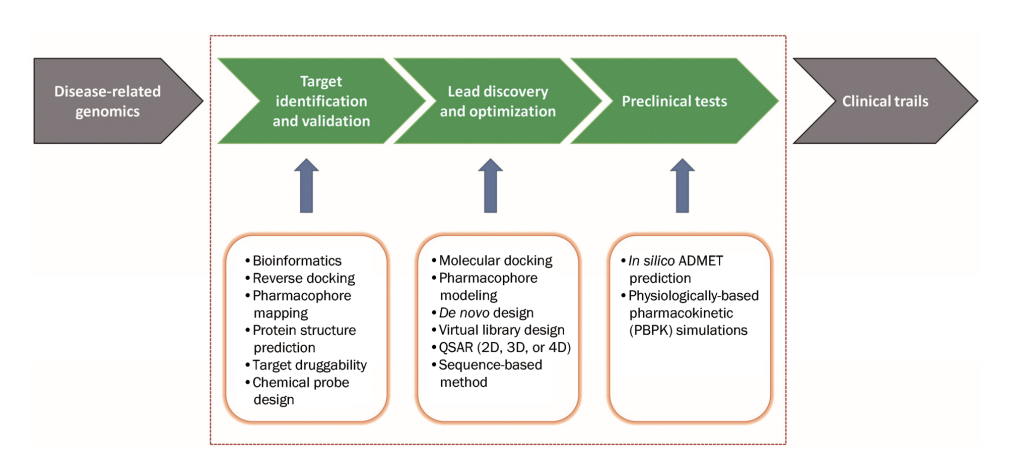
\includegraphics[scale=0.6]{siklus_dd.png}
	\caption{Diagram proses \textit{drug discovery} tradisional dan modern \cite{diagram drug discovery}}
\end{figure}
Dalam \textit{computational drug discovery} (penemuan obat dengan memanfaatkan komputer), pendekatan yang dapat dilakukan dibagi menjadi \textit{structure-based drug design} (SBDD), \textit{ligand-based drug design} (LBDD) dan pendekatan berdasarkan sekuens \cite{reviewCADD}. \textit{Structure-based drug design} (SBDD) terdiri dari proses \textit{docking} kandidat \textit{ligand} ke target \textit{receptor} kemudian dilakukan penilaian dengan menggunakan \textit{scoring function} untuk dapat menghitung kemungkinan \textit{ligand} tersebut terikat pada target protein dengan daya tarik yang tinggi \cite{rankingSBDD}. 
\begin{figure}
	\centering
	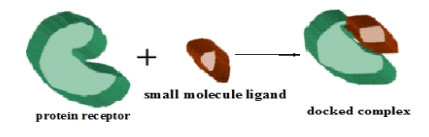
\includegraphics {molecular_docking.png}
	\caption{Ilustrasi \textit{ligand} yang akan terikat dengan \textit{receptor} \cite{gambar MolecularDocking}}
\end{figure}   
Dalam LBDD, diberikan sekumpulan \textit{ligand} dan \textit{receptor}, dimana model \textit{receptor} dapat dibuat dengan mengumpulkan informasi dari \textit{ligand} \cite{Drugdesign}. Model ini dikenal dengan \textit{pharmacophore}. Kemudian, kandidat \textit{ligand} akan dibandingkan dengan \textit{pharmacophore}, apakah kompatibel dengan \textit{pharmacophore} dan dapat terikat \cite{MolecularDocking}.
\begin{figure}
	\centering
	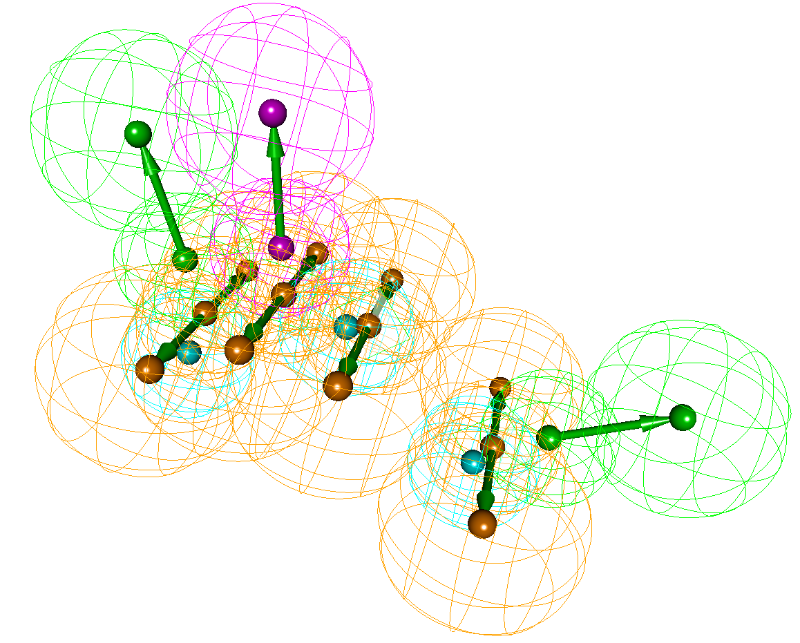
\includegraphics [scale=0.3]{pharmacophore.png}
	\caption{Contoh dari \textit{pharmacophore} \cite{pharmacophore}}
\end{figure}  

\section{\textit{Molecular Docking}}
%-----------------------------------------------------------------------------%

\hspace{0.5 cm}\textit{Virtual screening} berdasarkan \textit{molecular docking} merupakan metode yang sering digunakan dalam SBDD. Penulis juga akan menggunakan metode tersebut yang terdapat dalam aplikasi Autodock dan Autodock Vina. Pemodelan struktur kimia menggunakan \textit{molecular modeling} untuk mempelajari fenomena dari struktur kimia tersebut. Kemudahan dalam \textit{molecular modeling} sekarang ini dibantu dengan aplikasi komputer yang tersedia, namun masih terdapat kesulitan yaitu bagaimana cara mendapatkan model struktur ikatan kimia yang benar dan interpretasi model yang tepat. Secara umum, \textit{molecular modeling} dapat dikatakan sebagai pemanfaatan komputer dalam mengkonstruksi molekul dan melakukan berbagai macam perhitungan untuk mempelajari karakteristik dan sifat struktur ikatan kimia. Istilah \textit{molecular modeling} terkadang disamakan dengan istilah \textit{computational chemistry}.

Proses \textit{drug discovery} yang semula berupa \textit{trial and error} berubah menjadi proses yang dibantu dengan perhitungan komputer. Perhitungan tersebut digunakan dalam menentukan struktur ikatan kimia baru berdasarkan struktur protein yang sudah diketahui \cite{doCADD}. Pendekatan ini terbagi menjadi dua : \textit{de novo design} \cite{De Novo} dan \textit{docking} \cite{Docking and Scoring}. \textit{Docking} merupakan suatu proses untuk menebak struktur \textit{complex} dari struktur \textit{ligand} dan protein. Dalam \textit{molecular modeling}, \textit{docking} dapat dipandang sebagai suatu metode untuk memprediksi orientasi suatu molekul ketika diikat dengan molekul lainnya untuk membentuk \textit{complex} yang stabil.  
\begin{figure}
	\centering
	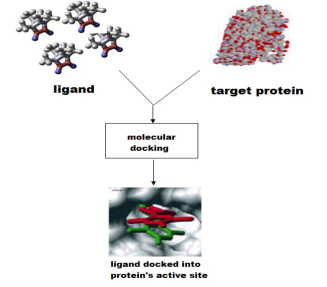
\includegraphics{docking.png}
	\caption{\textit{Proses molecular docking }\cite{MolecularDocking}}
\end{figure}

\textit{Molecular docking} adalah suatu proses komputasi dalam pencarian \textit{ligand} yang paling cocok baik secara geometri maupun energi ketika diikat dengan suatu \textit{receptor} (protein) yang telah diketahui \cite{MolecularDocking}. Aspek utama dalam \textit{molecular docking} adalah perhitungan energi interaksi dan konformasi dengan menggunakan metode dari kuantum mekanik hingga fungsi empiris energi. Permasalahan \textit{molecular docking} sekilas dapat dilihat sebagai suatu permasalahan \textit{lock and key}, dimana \textit{receptor} protein dapat dipandang sebagai \textit{lock} dan \textit{ligand} sebagai \textit{key}. Namun dalam praktiknya, \textit{molecular docking} akan mencari \textit{ligand} yang dapat menyesuaikan dengan \textit{receptor}. Karena adaptasi tersebut, \textit{molecular docking} dapat dipandang sebagai permasalahan "\textit{best-fit}" \textit{ligand} \cite{best-fit}. Diperlukan \textit{scoring function} untuk dapat membatasi \textit{best-fit} dari proses \textit{molecular docking}. Fungsi tersebut biasanya berdasarkan \textit{force field} yang digunakan dalam mensimulasikan protein. Beberapa \textit{scoring function} juga menambahkan aspek perhitungan lainnya seperti entropi \cite{MolecularDocking}.

Dalam percobaan ini penulis memanfaatkan aplikasi \textit{molecular docking} Autodock dan Autodock Vina dikarenakan kedua aplikasi tersebut sering dirujuk dalam karya ilmiah yang berkaitan dengan \textit{docking} \cite{autodock most cited}.

\section{\textit{Autodock dan Autodock Vina}}
%-----------------------------------------------------------------------------%
\hspace{0.5cm}Aplikasi ini merupakan aplikasi yang dikembangkan oleh \textit{The Scripps Research Institute}, lembaga riset nonprofit yang terletak di California, Amerika Serikat \cite{website resmi}. Terdapat 2 jenis aplikasi, Autodock dan Autodock Vina. Masing-masing merupakan aplikasi yang saling berbeda dalam segi \textit{scoring function} yang digunakan dan optimisasi komputasi secara paralel oleh Autodock Vina. Autodock memanfaatkan \textit{empirical free energy force field} dengan \textit{Lamarckian Genetic Algorithm} dalam  memprediksi koordinat ikatan antara \textit{ligand} dan \textit{receptor} \cite{autodock}. Sedangkan dalam Autodock Vina, dilakukan optimisasi dengan memanfaatkan \textit{particle swarm optimization} secara global dan \textit{Broyden-Fletcher-Goldfarb-Shanno (BFGS)} secara lokal \cite{autodockvina}. Pada percobaan ini penulis menggunakan Autodock versi 4.2 dan Autodock Vina versi 1.1.2.

Autodock versi 4.2 terdiri dari 2 program, Autodock4 dan Autogrid4. AutoGrid4 akan menghasilkan \textit{pre-calculated map} dari suatu \textit{ligand}. Selain itu juga akan menghasilkan \textit{map} tambahan, "d" untuk \textit{desolvation} dan "e" untuk \textit{electrostatic}. Pengoperasian Autodock membutuhkan beberapa file, yaitu : *.dpf untuk pengaturan \textit{docking} parameter , hasil \textit{map} berupa *.gpf dari AutoGrid , dan *.pdbqt untuk \textit{receptor} dan \textit{ligand} yang akan diujicoba. Keluaran yang dihasilkan oleh Autodock berupa *.dlg yang berisi hasil perhitungan konformasi posisi dan energi pada setiap \textit{ligand} yang diujicoba. Paket aplikasi Autodock Vina hanya datang dengan sebuah program saja dikarenakan bagian \textit{pre-processing docking} dibuat transparan sehingga pengguna tidak perlu tahu dan memahami bagaimana aplikasi tersebut bekerja. Autodock Vina membutuhkan 2 file, *.pdbqt dari \textit{ligand} dan *.pdbqt dari tiap \textit{receptor} yang akan diujicobakan. Keluaran yang dihasilkan juga berupa *.pdbqt yang beisikan konformitas posisi dan energi.
\begin{figure}
	\centering
	
\includegraphics{autodock.jpg}
	\caption{Logo Autodock \cite{Logo autodock}}
\end{figure}

\section{\textit{Kemampuan Komputasi}}
%-----------------------------------------------------------------------------%
\textit{Molecular docking} yang dilakukan antara suatu \textit{ligand} dan \textit{receptor} akan menentukan apakah \textit{ligand} tersebut merupakan calon dari obat yang sedang dicari. Dengan bermunculan berbagai aplikasi yang membantu dalam proses molecular docking, kesulitan ketika melakukan secara manual dengan menggunakan alat peraga akan berkurang serta perhitungan dan tingkat presisi akan lebih baik dibandingkan dengan perhitungan manusia. Kompleksitas dari \textit{ligand } dan \textit{receptor} juga akan mempengaruhi evaluasi fungsi yang dikerjakan dalam aplikasi \textit{molecular docking}\cite{MolecularDocking}.

\textit{Virtual screening} merupakan suatu teknik komputasi yang dilakukan dalam \textit{drug discovery} dimana secara otomatis akan mengevaluasi kumpulan bank data \textit{receptor} dengan suatu \textit{ligand} untuk menentukan calon obat \cite{virtual screening}. Dibutuhkan kemampuan komputasi yang dapat menjalankan eksekusi perintah dengan cepat. CPU, sebagai pusat pengolah data dan instruksi pada komputer membutuhkan \textit{clock rate} yang cepat dan kemampuan menjalankan instruksi per \textit{clock} yang besar. Terlepas dari kompleksitas molekul \textit{ligand} maupun \textit{receptor}, faktor tersebut mengambil peranan penting dalam riset yang memanfaatkan kemampuan komputasi.

Muncul infrastruktur yang dapat dikatakan memiliki kesamaan dengan \textit{supercomputer}, \textit{Computer Cluster}. \textit{Computer Cluster} dapat dikatakan sebagai komputer yang saling berhubung dan dipandang sebagai satu kesatuan. Setiap anggota (\textit{cluster}) akan mengerjakan perintah yang sama diatur dalam \textit{software} penjadwalan. \textit{Cluster} ini dapat membantu peneliti dalam mengerjakan risetnya dengan performa yang tidak berbeda dengan \textit{supercomputer} \cite{cluster_pak hilman}. Berbeda dengan \textit{cluster}, muncul istilah \textit{grid computing}, dimana secara struktur mirip dengan \textit{cluster}, namun untuk setiap bagian komputer mengerjakan tugas yang berbeda beda (namun dalam satu tujuan) \cite{grid}.
  
\section{\textit{Cloud Computing}}
%-----------------------------------------------------------------------------%
\hspace{0.5cm}Teknologi \textit{cloud computing} sudah berkembang sejak tahun 1990-an. Pada awalnya teknologi ini dikembangkan sebagai solusi dari permasalahan yang dihadapi oleh perusahaan dengan bertambahnya kapasitas data yang perlu disimpan dan pengeluaran yang cukup besar untuk pengadaan perangkat keras beserta konsumsi daya listrik yang dibutuhkan \cite{Cloud Computing: Overview and Risk Analysis}. Definisi dari \textit{cloud computing} dapat dikatakan sebagai virtualisasi dari perangkat komputasi, dimana pengguna mengakses perangkat tersebut dengan menggunakan jaringan internet \cite{Cloud Computing Research and Development Trend}. Selain itu, teknologi ini memberikan kemudahan dalam penggunaan secara \textit{multiuser}, dimana dapat diakses secara bersamaan.

Terdapat 3 karakteristik dari teknologi \textit{cloud computing}, yaitu virtualisasi, terdistribusi, dan kemudahan dalam pengembangan selanjutnya (\textit{dynamically extendibility}). Virtualisasi merupakan faktor yang utama. Virtualisasi dapat membagi suatu perangkat komputasi secara fisik menjadi beberapa "virtual" perangkat komputasi. Dengan begitu, kinerja dari perangkat akan dioptimisasi. Alokasi sumber daya perangkat keras tidak ada yang diam secara percuma. Disamping itu, dengan adanya virtualisasi dapat menekan biaya pengeluaran pengadaan perangkat komputasi secara fisik. Yang dimaksud dengan terdistribusi adalah perangkat keras (\textit{physical node}) yang digunakan dalam \textit{cloud computing} digunakan secara terdistribusi. Dalam tahap pengembangan teknologi ini memberikan kemudahan. Kemudahan tersebut merupakan efek dari virtualisasi. Ketika pengguna ingin mengikuti perkembangan yang ada, tidak perlu merubah / membuat kembali dari awal. Pengguna dapat merubah dari level virtual (virtualisasi).


Terdapat 3 jasa yang disediakan dalam \textit{cloud computing} \cite{Cloud Computing Research and Development Trend} :
\begin{itemize}
	\item \textbf{Software as a Service (SaaS)}\\
	Layanan jasa ini menyediakan aplikasi dan penyimpanan data (\textit{database}) yang langsung dapat digunakan. Pengguna dapat mengakses aplikasi secara bersamaan dengan pengguna lainnya. SaaS dikenal juga sebagai \textit{on-demand software} dan biaya yang dikenakan oleh penyedia jasa ini merupakan \textit{pay-per-use}. Umumnya, pengguna akan dikenakan biaya bulanan atau tahunan. Pengguna tidak perlu susah - susah untk menginstall aplikasi pada \textit{cloud} dikarenakan penyedia jasa tersebut akan melakukan hal tersebut. Saas memberikan keuntungan bagi perusahaan dengan cara mengurangi biaya operasional IT (Information Technology). Hal ini dikarenakan biaya untuk pemeliharaan dan pengadaan perangkat komputasi ditanggungkan kepada pihak penyedia jasa (\textit{outsourcing}). Contoh dari Saas adalah layanan \textit{e-mail}, media sosial.
	
	\item \textbf{Platform as a Service (PaaS)}\\
	Berbeda dengan Saas, layanan ini menyediakan perangkat komputasi yang dapat digunakan untuk menjalankan aplikasi dari pengguna. Layanan ini dapat menyediakan sistem operasi atau \textit{framework} yang dibutuhkan dalam menjalankan apliksi tersebut. Contoh dari layanan jasa ini adalah : Windows Azure, Amazon Web Service, dan Google App Engine.
	
	\item \textbf{Infrastructure as a Service (IaaS)}\\
	layanan ini menyediakan infrastruktur IT kepada pengguna sesuai dengan permintaan yang dapat diakses dengan jaringan internet. Infrstruktur tersebut meliputi perangkat keras seperti \textit{harddisk, memory, firewall}, tipe server, alamat IP, \textit{virtual local area networks}(VLANs), maupun aplikasi yang harus terinstall dalam server 
	  
\end{itemize}
\begin{figure}
	\centering
	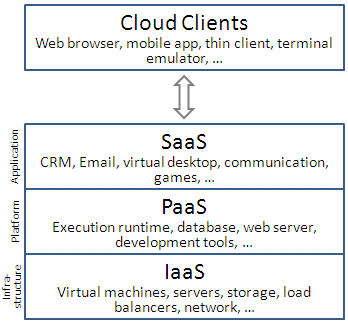
\includegraphics[scale=0.6]{layanan_cloud.png}
	\caption{Layanan dalam \textit{cloud computing} \cite{Layanan cloud}}
\end{figure}

\section{Virtualisasi}
%-----------------------------------------------------------------------------%
\hspace{0.5cm}Virtualisasi merupakan suatu konsep dimana suatu sistem komputer secara nyata dapat dijalankan lebih dari satu / \textit{multiple} pada suatu \textit{host}. Virtualisasi bisa berjalan dengan adanya VMM (\textit{Virtual Machine Monitor}) yang mengatur komunikasi antara lingkungan virtualisasi dengan perangkat keras. Virtualisasi juga dapat dipandang sebagai teknik optimisasi perangkat keras sebagai sumber komputasi \cite{vmm}. Terdapat 3 arsitektur dari VMM :
\begin{itemize}
	\item \textbf{Full Virtualization} \\ Pada tipe ini, \textit{hypervisor} dapat menjalankan beberapa sistem komputer virtual secara bersamaan. Setiap komputer virtual tersebut tidak perlu tahu bahwa mereka berjalan dalam lingkungan virtual
	\item \textbf{Para Virtualization} \\ Dalam tipe ini, sedikit modifikasi dilakukan dari Full Virtualization, dimana setiap sistem komputer virtual sadar bahwa mereka berjalan dalam lingkungan virtual dan sadar dengan keberadaan sistem komputer virtual lainnya. Selain itu, untuk setiap aplikasi yang dieksekusi pada masing - masing sistem komputer virtual akan langsung diteruskan ke perangkat keras tanpa harus melalui Virtual Machine Monitor
	\item \textbf{OS Partitioning} \\ Dalam tipe ini , virtualisasi dilakukan pada level OS, dimana \textit{hypervisor} terinstall pada masing masing OS pada sistem komputer virtual yang diinstall diatas OS host. Batasan dalam tipe ini adalah, OS pada sistem komputer virtual harus mengikuti OS pada host.
\end{itemize}

   
\hspace{0.5cm}Virtualisasi digunakan pada teknologi \textit{cloud computing} dalam mengoptimisasi kinerja server sehingga tidak ada sumber daya yang tidak terpakai. Virtualisasi yang dimaksud adalah virtualisasi perangkat keras (\textit{hardware}) \cite{Virtualization in Education}. Virtualisasi tersebut  memungkinkan "virtual" server yang dapat dibuat sesuai dengan kebutuhan yang diperlukan dan berjalan pada server fisik. Spesifikasi untuk masing - masing virtual server dapat disesuaikan dengan kebutuhan aplikasi yang akan dijalankan diatasnnya dan tidak melebihi spesifikasi server fisik. Masing - masing virtual server akan saling terisolasi satu dengan yang lainnya. 

Permasalahan virtualisasi tersebut muncul ketika hendak mengoptimisasikan sumber daya yang ada. Ketika suatu "virtual" server dibuat untuk menjalankan suatu aplikasi yang spesifik, maka keseluruhan sistem perlu dibuat (Sistem operasi, alokasi sumber daya memori, \textit{processor}) termasuk \textit{library} yang dibutuhkan dalam menjalankan sistem / aplikasi tersebut. "virtual" server tersebut akan diatur oleh suatu program VMM yang menjembatani komunikasi dengan server fisik. Dengan begitu, kapasitas memori dan alokasi sumber daya pada server tidak optimal dalam menjalankan "virtual" server secara bersamaan.

\section{Virtual Machine}
%-----------------------------------------------------------------------------%
Definisi dari \textit{virtual machine} sendiri adalah suatu aplikasi atau \textit{operating system} yang berjalan pada suatu aplikasi yang mengimitasi \textit{hardware} asli yang sesuai dengan lingkungan aplikasi atau \textit{operating system} tersebut. Pada umumnya virtualisasi yang sering digunakan adalah \textit{full virtualization}, dimana terdapat suatu program tersendiri (\textit{hypervisor}) yang mengatur \textit{virtual machine} dengan pembagian \textit{resource} hardware asli (\textit{virtual machine} dapat dikatakan sebagai \textit{guest} dan tempat dimana \textit{virtual machine} diinstall dapat dikatakan sebagai \textit{host}). Masing - masing \textit{virtual machine} yang berjalan pada host akan terisolasi satu dengan lainnya, namun \textit{resource} hardware \textit{host} akan terbagi satu sama lain. terdapat 2 tipe \textit{hypervisor} :
\begin{itemize}
	\item \textbf{Type 1} \\ Pada tipe ini, \textit{hypervisor} langsung terinstall pada \textit{hardware} dan berfungsi untuk mengatur \textit{hardware} dan \textit{operating system} yang terinstall diatasnya (\textit{virtual machine})
	\item \textbf{Type 2} \\ Berbeda dengan tipe sebelumnya, \textit{hypervisor} terinstall pada \textit{operating system guest} dimana \textit{virtual machine} terinstall layaknya suatu program.
\end{itemize}

Umumnya \textit{hypervisor} tipe 2 sering digunakan pada komputer - komputer konvensional. Contoh aplikasi ini adalah VMWare\cite{vmware} maupun VirtualBox \cite{virtualbox}.

Kebutuhan virtualisasi pada awalnya merupakan suatu cara untuk memberikan kemudahan dalam meng\textit{install operating system} pada mesin - mesin yang sudah lama. Selain itu, dengan virtualisasi kita dapat meng\textit{install} berbagai \textit{operating system} dalam sebuah mesin tanpa harus takut pengaturan tiap - tiap \textit{operating system} akan saling mempengaruhi \textit{operating system} lainnya (prinsip virtualisasi dimana setiap \textit{virtual machine} akan saling tertutup dengan \textit{virtual machine} lainnya). Selain itu, seperti yang digunakan dalam \textit{cloud computing}, virtualisasi mengoptimalkan pemanfaatan \textit{resource} hardware untuk meningkatkan layanan. Sebagai contoh, para developer akan menguji sistem atau aplikasi yang telah dibuat pada \textit{environtment} sebenarnya, sehingga diperlukan suatu wadah uji coba yang sesuai dengan sistem atau aplikasi tersebut. Dengan adanya teknik virtualisasi tersebut, baik dengan \textit{cloud computing} maupun pada komputer sendiri, developer tidak perlu takut sistem atau aplikasi yang dijalankan akan menyebabkan kerusakan pada \textit{environment} dan berdampak juga pada pekerjaan sebelumnya.

Teknik \textit{full virtualization} juga memiliki kekurangan. Untuk mengoptimalkan kinerja \textit{host} dalam meningkatkan kualitas aplikasi yang berjalan pada \textit{virtual machine} (\textit{guest}). Untuk membentuk sebuah \textit{guest}, \textit{hypervisor} akan membutuhkan data memori, prosesor, jaringan yang \textit{fixed}. Dengan begitu, jumlah \textit{virtual machine} yang akan terbentuk akan terikat dengan besarnya \textit{resource} hardware yang dimiliki oleh \textit{guest}. Disatu sisi, ketika suatu \textit{virtual machine} sedang menjalankan proses yang membutuhkan kemampuan komputasi tambahan, \textit{hypervisor} tidak dapat memberikan \textit{resource} tambahan, walaupun \textit{virtual machine} lainnya dalam keadaan \textit{idle} (tidak bekerja). 

      
\section{Docker}
%-----------------------------------------------------------------------------% 
\hspace{0.5cm}Docker, \textit{platform} virtualisasi yang dikembangkan oleh Perusahaan Docker menggunakan teknik berbeda dengan \textit{Full Virtualization}. Docker menggunakan \textit{Docker engine} sebagai ganti dari \textit{hypervisor}. \textit{Docker engine} dikembangkan berdasarkan \textit{Linux containers} (LXC), dimana level virtualisasi terletak pada sistem operasi \cite{LXC} (bentuk virtualisasi \textit{OS Partitioning}). Dengan begitu suatu server linux dapat menjalankan beberapa sistem linux yang saling terisolasi satu sama lain. Kernel pada "virtual" server, dalam hal ini disebut container yang dibentuk dengan libcontainer \cite{libcontainer} akan menggunakan kernel yang sama dengan server fisik. Oleh karena itu, container yang dibentuk akan lebih kecil dan padat tanpa perlu menginstall sistem secara keseluruhan dari awal. container tidak perlu mengalokasikan sumber daya secara tetap dikarenakan \textit{Docker engine} akan mengalokasikan sumber daya berdasarkan aplikasi yang berjalan pada container \cite{VMware and Docker – Better Together}.
\begin{figure}
	\centering
	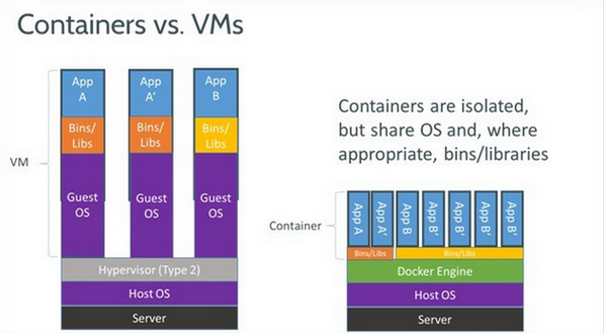
\includegraphics[scale=0.6]{vm.png}
	\caption{Perbandingan virtualisasi pada VM dan \textit{container} pada Docker\cite{vmmvscontainer}}
\end{figure}

\begin{figure}
	\centering
	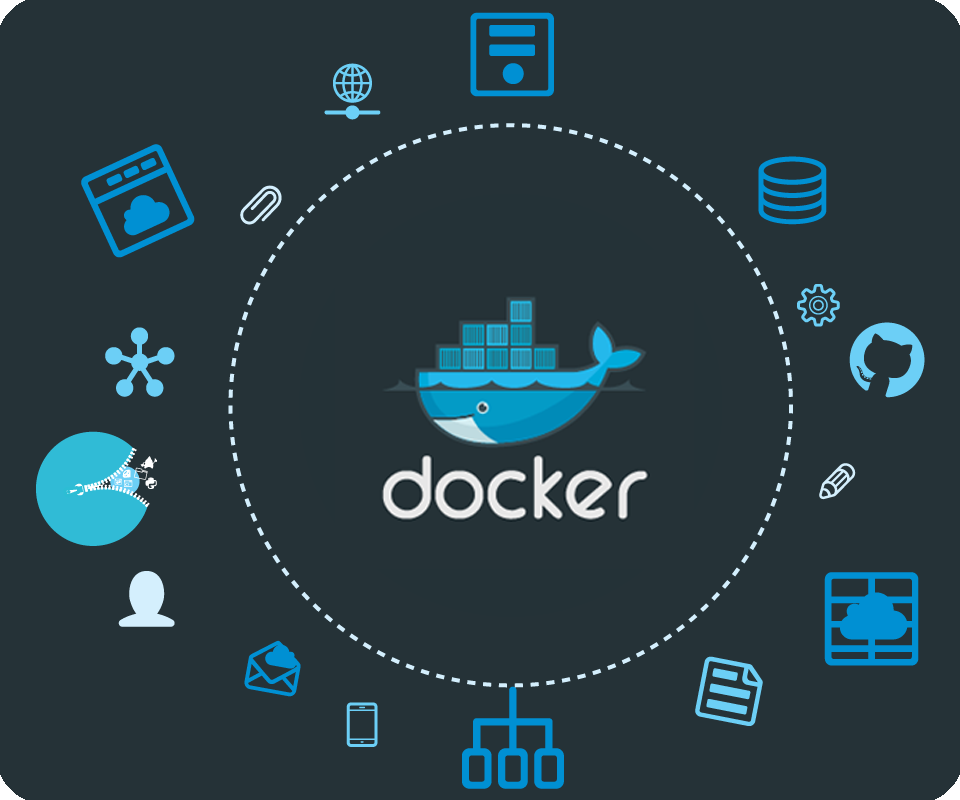
\includegraphics[scale=0.8]{docker.png}
	\caption{Logo Docker\cite{Logo Docker}}
\end{figure}

Walaupun begitu, untuk masing masing virtualisasi, baik itu yang menggunakan \textit{hypervisor} maupun \textit{Docker engine} pada Docker memiliki kelebihan dan kekurangan masing - masing. \textit{Container} yang dibentuk pada Docker harus menggunakan sistem operasi yang sama dengan server fisik. Untuk saat ini, Docker baru mendukung sistem operasi Linux sebagai \textit{container} dan berjalan pada sistem operasi Linux. Walaupun dapat berjalan pada sistem operasi lainnya, namun penggunaan Docker masih dijalankan dalam "virtual" komputer yang menggunakan sistem operasi Linux pada \textit{Virtual Machine}. Dengan alokasi sumber daya yang tidak tetap (sesuai dengan proses yang berjalan), maka \textit{container} yang terbentuk akan lebih banyak dari "virtual" server yang dihasilkan dengan menggunakan "hypervisor" pada umumnya terikat dengan batasan sumber daya. Namun "virtual" server tersebut lebih beragam dan tidak terikat dengan sistem operasi yang berjalan pada server fisik.   
         